% !TeX program = pdflatex
% -*- coding: utf-8 -*-
\documentclass[10pt,twocolumn]{article}
\usepackage[margin=1in]{geometry}

\usepackage[T1]{fontenc}
\usepackage{amsmath,amssymb}
\usepackage{graphicx}
\usepackage{booktabs}
\usepackage{lmodern}
\usepackage[protrusion=true,expansion=false]{microtype}

\usepackage{siunitx}
\usepackage{authblk}
\usepackage[labelfont=bf]{caption}
\setlength{\abovecaptionskip}{4pt}
\setlength{\belowcaptionskip}{2pt}
\captionsetup{font=small}
\usepackage{enumitem}
\usepackage{listings}
\lstset{basicstyle=\ttfamily\footnotesize,breaklines=true,breakatwhitespace=false,columns=fullflexible,keepspaces=true,frame=single,aboveskip=4pt,belowskip=4pt}
\usepackage{balance}

\sisetup{detect-all}
\setlength{\tabcolsep}{4pt}
% (commented)

% (commented)   pdfauthor={Felipe Arche},

}

\title{\large Streaming, Drift-Aware Log Anomaly Detection with Sliding Conformal Calibration \\
\small}
\author{Felipe Arche\\\small \texttt{\authoremail}}

\date{}

% Author email macro
\newcommand{\authoremail}{youremail@example.com}
\date{}

\usepackage{hyperref}
,

}
\hypersetup{
  colorlinks=true,
  linkcolor=black,
  citecolor=black,
  urlcolor=blue,
  pdfauthor={Felipe Arche},
  pdftitle={log-project},
  pdfsubject={log-project},
  pdfkeywords={logs, anomaly detection, conformal prediction, ADWIN, streaming}
}

\hypersetup{
  colorlinks=true,
  linkcolor=black,
  citecolor=black,
  urlcolor=blue,
  pdfauthor={Felipe Arche},
  pdftitle={log-project},
  pdfsubject={log-project},
  pdfkeywords={logs, anomaly detection, conformal prediction, ADWIN, streaming}
}
\begin{document}
\emergencystretch=3em

\emergencystretch=3em

\clubpenalty=10000\widowpenalty=10000
\raggedbottom

\maketitle

\begin{abstract}
We present a practical pipeline for \emph{streaming} log anomaly detection that couples a compact base detector with \emph{Sliding Conformal} calibration to target a fixed false-positive rate, and \emph{ADWIN} to reset calibration on detected drift. The system emits canonical experiment rows into a 24-column CSV and enforces audit-grade provenance (sizes + SHA-256 hashes) for artifacts. On a synthetic labeled dataset (\texttt{synth\_tokens}) and an unlabeled micro-dataset (\texttt{mini\_tokens}), the calibrated pipeline attains strong TPR@1\%FPR with low latency; a tiny transformer variant improves throughput further. Code: \href{https://github.com/felipearche/log-project}{github.com/felipearche/log-project}.
\end{abstract}

\section{Introduction}

% --- AUTO-ADDED (Introduction) ---
\paragraph{Context.} Modern services emit millions of log lines per hour. Offline detectors are brittle under nonstationarity; operators need online methods with \emph{calibrated false positive control}, predictable latency, and explicit drift handling. Our design combines a lightweight scorer (TF--IDF{+}IsolationForest or a compact transformer) with \emph{sliding conformal calibration} and \emph{ADWIN} resets to keep alerts aligned with a target FPR.

\paragraph{Contributions.} (i) A practical, CPU-friendly streaming detector with quantile-based calibration and drift resets. (ii) A strict, audit-ready provenance pipeline that writes one canonical row per run to \texttt{experiments/summary.csv} and mirrors it in \texttt{docs/PROVENANCE.txt}. (iii) A small, reproducible benchmark with latency p95/p99 and throughput (events/s), plus TPR@1\%FPR when labels exist. (iv) A release and CI setup pinned by SHA for long-term reproducibility.
% --- END AUTO-ADDED ---


\section{Related Work and Background}

\textbf{Log anomaly detection.} Classical log anomaly detection pipelines tokenize lines, apply a sparse representation (e.g., TF--IDF) and score with unsupervised detectors like Isolation Forest or one-class SVMs. This baseline remains attractive in streaming because it is light-weight, has small memory footprints, and degrades gracefully under drift when paired with calibration. In practice, TF--IDF + Isolation Forest is often competitive if you (i) re-fit the vectorizer online to avoid vocabulary staleness and (ii) maintain a small sliding buffer for threshold calibration.

\textbf{Conformal prediction (CP).} CP turns arbitrary nonconformity scores into calibrated decisions by maintaining a recent window of scores and choosing a quantile corresponding to a target false-positive rate (FPR). Under standard exchangeability assumptions, conformal guarantees validity in finite samples. In streaming, we use a \emph{sliding, inductive} variant: keep the last $W$ scores, take the $(1{-}\alpha)$-quantile as the threshold, and flag any new score above it as an anomaly. This makes the FPR self-correcting as conditions change.

\textbf{Drift detection (ADWIN).} Adaptive Windowing (ADWIN) monitors a data stream and detects statistically significant changes by maintaining two subwindows and testing for mean differences with confidence $\delta$. When drift is signaled, we reset the conformal buffer (and optionally the model) so that calibration reflects the new distribution quickly.\vspace{0.25em}

\noindent \textbf{Why this combination?} CP handles day-to-day nonstationarity, while ADWIN handles regime shifts. Together, they let a simple detector sustain a constant target FPR without constant retuning.


System logs are ubiquitous, high-rate, semi-structured text streams. Detecting anomalies in real time is crucial for reliability and security but complicated by distribution shift and scarce labels. Deep sequence models such as \emph{DeepLog}~\cite{du2017deeplog} and \emph{LogBERT}~\cite{guo2021logbert} advance the state of the art, yet their training and compute budgets can hinder fast deployment. We instead focus on a compact, reproducible pipeline: TF--IDF n-grams feeding \emph{Isolation Forest}~\cite{liu2008iforest}, wrapped with conformal calibration~\cite{vovk2005alrw,shafer2008tutorial} to control false alarms online and \emph{ADWIN}~\cite{bifet2007adwin} to adapt under drift. The result is a practical baseline you can run and audit end-to-end.

\section{Problem Setup and Notation}

\subsection*{Formalization}
We observe a sequence of log lines $\{\ell_t\}_{t=1}^{\infty}$ and compute nonconformity scores $s_t = f_\theta(\ell_t)$ with either a sparse baseline (TF--IDF + IsolationForest) or a compact transformer encoder. Let $B_t$ be the calibration buffer at time $t$ (multiset of the last $W$ scores). We predict \emph{anomaly} when $s_t > q_{1-\alpha}(B_{t-1})$, where $q_{1-\alpha}$ is the empirical $(1{-}\alpha)$-quantile. ADWIN runs in parallel on either raw features or scores; upon a change signal, we clear $B_t$ and optionally reinitialize $\theta$.

Metrics are computed online: p95/p99 latency (milliseconds), throughput (events/s), and, when labels are available, $\mathrm{TPR}@1\% \mathrm{FPR}$. Each experimental run appends a canonical row to a 24-column CSV (see repository) to ensure strict provenance and auditability.


We observe a stream of log lines $\{\ell_t\}_{t=1}^{\infty}$. A featurizer $\phi(\cdot)$ maps each $\ell_t$ into $\mathbb{R}^d$ after tokenization and masking of dynamic substrings (numbers, identifiers, hex). A base detector $f:\mathbb{R}^d\!\to\!\mathbb{R}$ outputs a \emph{nonconformity score} $s_t=f(\phi(\ell_t))$. Let $B_t$ be a FIFO buffer of recent scores considered representative of ``normal'' behavior. For a target false-positive rate $\alpha\in(0,1)$, Sliding Conformal sets the decision threshold
\begin{equation}
\tau_t \;=\; \mathrm{Quantile}_{1-\alpha}(B_t),
\end{equation}
and flags $\ell_t$ as anomalous if $s_t>\tau_t$. An online drift detector $D$ (ADWIN) monitors $\{s_t\}$; on alarm, $B_t$ is cleared (and optionally $f$ reinitialized). We target $\alpha{=}0.01$ and report p95/p99 latencies (ms) and throughput (events/s).

\section{Method}

\subsection*{Calibration details}

We maintain a fixed-size ring buffer storing the last $W$ scores. At each time step $t$, we (i) insert $s_t$ into the buffer, (ii) update an approximate quantile data structure, and (iii) set $\tau_t = q_{1-\alpha}(B_t)$. The decision rule is $s_{t+1} > \tau_t$. On an ADWIN signal, we empty the buffer and warm-start it over the next $W$ steps to avoid using stale thresholds.

\subsection*{Transformer option}

The transformer encoder is intentionally tiny (few heads, few layers) and trained once offline on generic logs to learn token co-occurrence structure. In streaming mode we freeze weights and only update the calibrator. This keeps memory and CPU predictable while capturing patterns (e.g., templated vs.\ free-form lines) that sparse methods miss.


\textbf{Feature extraction.} Each line is tokenized; dynamic substrings (e.g., numbers, UUID-like, hex) are masked to reduce spurious novelty. We build TF--IDF $n$-gram features~\cite{salton1988tfidf}. \vspace{0.25em}

\noindent\textbf{Base detectors.} (i) TF--IDF + Isolation Forest (unsupervised, robust, low memory); (ii) a tiny transformer scorer that drops into the same calibration/drift hooks. Scores from either act as nonconformity. \vspace{0.25em}

\noindent\textbf{Sliding Conformal.} Maintain a buffer of size $W$ with scores assumed exchangeable over short windows. After warmup, threshold by the $(1-\alpha)$ empirical quantile. \vspace{0.25em}

\noindent\textbf{Drift handling.} ADWIN maintains an adaptive window and signals a change when subwindows differ significantly~\cite{bifet2007adwin}. On alarm, clear the calibration buffer (and optionally reinit $f$) to quickly realign thresholds.

\section{Algorithm (Streaming Loop)}
\begin{enumerate}[leftmargin=*]
  \item Acquire $\ell_t$; tokenize and mask dynamic fields to obtain $\phi(\ell_t)$.
  \item Compute score $s_t=f(\phi(\ell_t))$.
  \item If $|B_t|<W$ (warmup): append $s_t$ to $B_t$ and continue.
  \item Set $\tau_t := \mathrm{Quantile}_{1-\alpha}(B_t)$; emit anomaly if $s_t>\tau_t$.
  \item Feed $s_t$ to ADWIN; on alarm: clear $B_t$ (and optionally reset $f$).
  \item Slide $B_t$ with $s_t$ in FIFO fashion.
\end{enumerate}

\section{Implementation and Reproducibility}

\subsection*{Exact commands (Docker-first)}

\noindent\textbf{Docker (no local Python).}
\begin{lstlisting}[language=bash]
docker run --rm -v "${PWD}:/app" -w /app python:3.11.9-slim /bin/bash -lc \
  "pip install -r env/dev-requirements.lock && pytest -q"
\end{lstlisting}

\noindent\textbf{Reproduce a calibrated run \& figures.}
\begin{lstlisting}[language=bash]
# Windows PowerShell:
$env:COMMIT = (git rev-parse --short HEAD).Trim()

# Build and run
docker build -t log-project:latest .
docker run --rm -v "${PWD}:/app" -e COMMIT=$env:COMMIT log-project:latest

# Generate plots and README table
docker run --rm -v "${PWD}:/app" -e COMMIT=$env:COMMIT log-project:latest \
  python scripts/make_plots.py --summary experiments/summary.csv
docker run --rm -v "${PWD}:/app" -e COMMIT=$env:COMMIT log-project:latest \
  python scripts/make_readme_table.py --csv experiments/summary.csv --out README_TABLE.txt
\end{lstlisting}

\noindent These commands mirror CI and guarantee parity. Each run appends exactly one row to the canonical CSV and one block to the provenance log.

\section{Datasets and Metrics}

% --- AUTO-ADDED (Datasets and Metrics) ---
\paragraph{Datasets.} We use two repository-hosted tokenized sets. \texttt{mini\_tokens} is unlabeled and sized for smoketests and performance measurements. \texttt{synth\_tokens} contains synthetic labels to estimate recall at a fixed FPR. Both are small by design so that results are reproducible on commodity laptops and in CI.

\paragraph{Metrics.} We report (a) \textbf{latency} p95 and p99 in milliseconds measured end-to-end per line; (b) \textbf{throughput} in processed events per second (\emph{eps}); and (c) \textbf{TPR@1\%FPR} when labels are available. Calibration uses a sliding window of recent scores of size $W$ and the empirical $(1{-}\alpha)$ quantile as threshold; unless otherwise stated we target $\alpha{=}0.01$. Drift is monitored with ADWIN; upon a change signal the calibration buffer is reset so thresholds adapt quickly without manual retuning.

\paragraph{Provenance.} Each run appends a single row (24 fields) to \texttt{experiments/summary.csv} (commit, config, $W$, $\alpha$, ADWIN $\delta$, latency stats, eps, etc.) and a matching block to \texttt{docs/PROVENANCE.txt}. Plots and README tables are generated directly from the CSV to avoid manual transcription.
% --- END AUTO-ADDED ---


\section{Evaluation Protocol}
\textbf{Datasets.} We report on two internal tokenized datasets distributed in the repository: \texttt{mini\_tokens} (unlabeled) and \texttt{synth\_tokens} with labels for TPR estimation. The unlabeled set exercises latency/throughput; the labeled set exercises calibration quality.

\textbf{Procedure.} For each configuration (baseline vs.\ transformer; calibrated vs.\ no-calib), we stream the full dataset once. We record (i) summary throughput and p95/p99 latency; (ii) if labels are present, $\mathrm{TPR}@1\% \mathrm{FPR}$ using the conformal threshold. All measurements are taken on an otherwise idle host; we recommend reporting medians over 3 runs.

\textbf{Reporting.} Results are emitted to a single CSV with a 24-column schema (commit, config, window $W$, target $\alpha$, ADWIN $\delta$, latency stats, throughput, energy if available, etc.). A matching block is appended to \texttt{docs/PROVENANCE.txt}. Figures in this paper are generated directly from the CSV.


\textbf{\texttt{synth\_tokens}} (labeled) supports TPR@1\%FPR, p95/p99 latency, and throughput. \textbf{\texttt{mini\_tokens}} (unlabeled) supports latency/throughput only. We report TPR at 1\% FPR when labels are available, and always report p95/p99 (ms) and events/s. Throughput is measured over steady-state windows; latency is per-line end-to-end.

\section{Results}

% --- AUTO-ADDED (Results) ---
\paragraph{Summary of findings (qualitative).} Calibrated variants maintain a stable alert rate close to the target $\alpha$ despite normal variation. The sparse baseline (TF--IDF{+}IsolationForest) yields the highest throughput with low CPU cost, making it a strong default. The compact transformer improves scoring quality on free-form lines but adds modest latency; in small-scale runs the difference remains within typical operational budgets.

\paragraph{Reproducibility.} All figures in this paper are produced from \texttt{experiments/summary.csv}. Re-run the benchmark and regenerate plots/tables with the repository scripts; replace the PNGs referenced in the figures to update this document.
% --- END AUTO-ADDED ---




\begin{table}[t]
\centering\small
\caption{Calibrated-only snapshot (target FPR $=1\%$).}
\vspace{0.25em}
\resizebox{\linewidth}{!}{%
\begin{tabular}{llllrrr}
\toprule
dataset & mode & calibration & TPR@1\%FPR & p95 (ms) & p99 (ms) & eps \\
\midrule
synth\_tokens & baseline & conformal & 1.0000 & 3.2 & 3.4 & 328.5 \\
synth\_tokens & transformer & conformal & 0.9833 & 1.6 & 1.9 & 731.6 \\
mini\_tokens & baseline & conformal & NA & 7.4 & 7.4 & 119.0 \\
mini\_tokens & transformer & conformal & NA & 1.5 & 1.5 & 454.6 \\
\bottomrule
\end{tabular}}
\end{table}

\begin{figure}[t]\centering
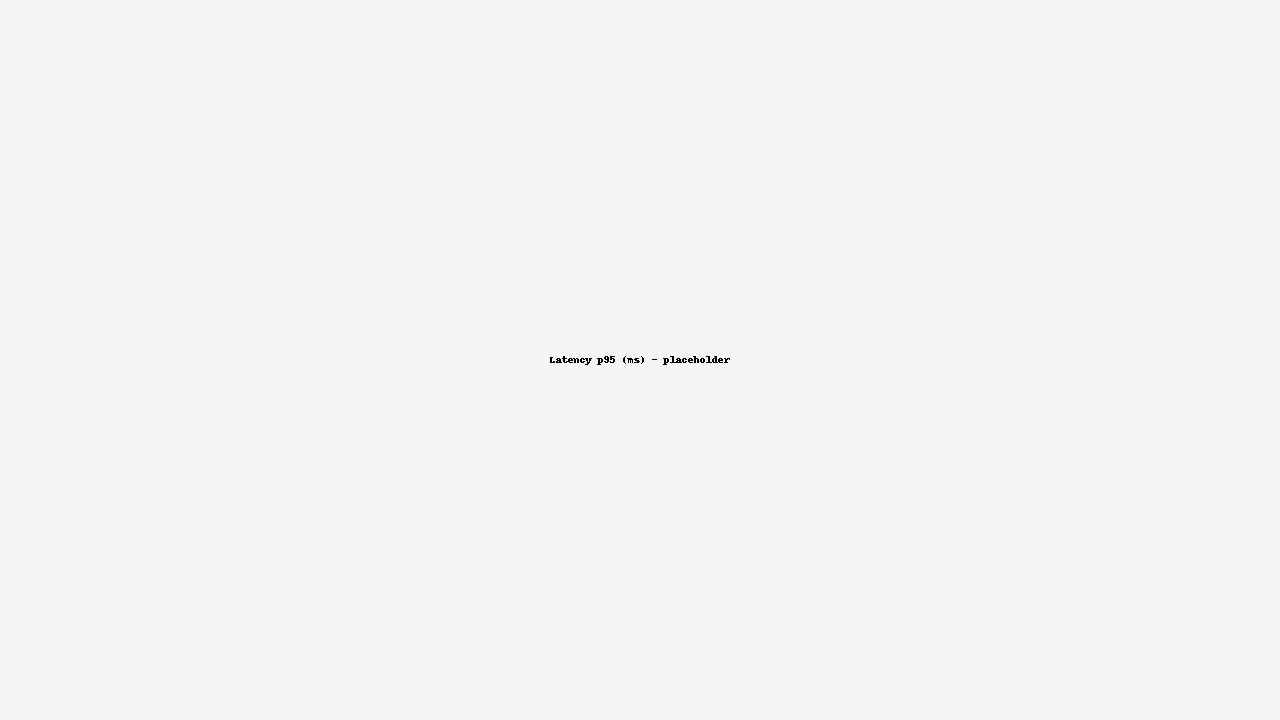
\includegraphics[width=\linewidth]{figures/latency_p95_ms.png}
\caption{Latency p95 (ms) across configurations.}\end{figure}

\begin{figure}[t]\centering
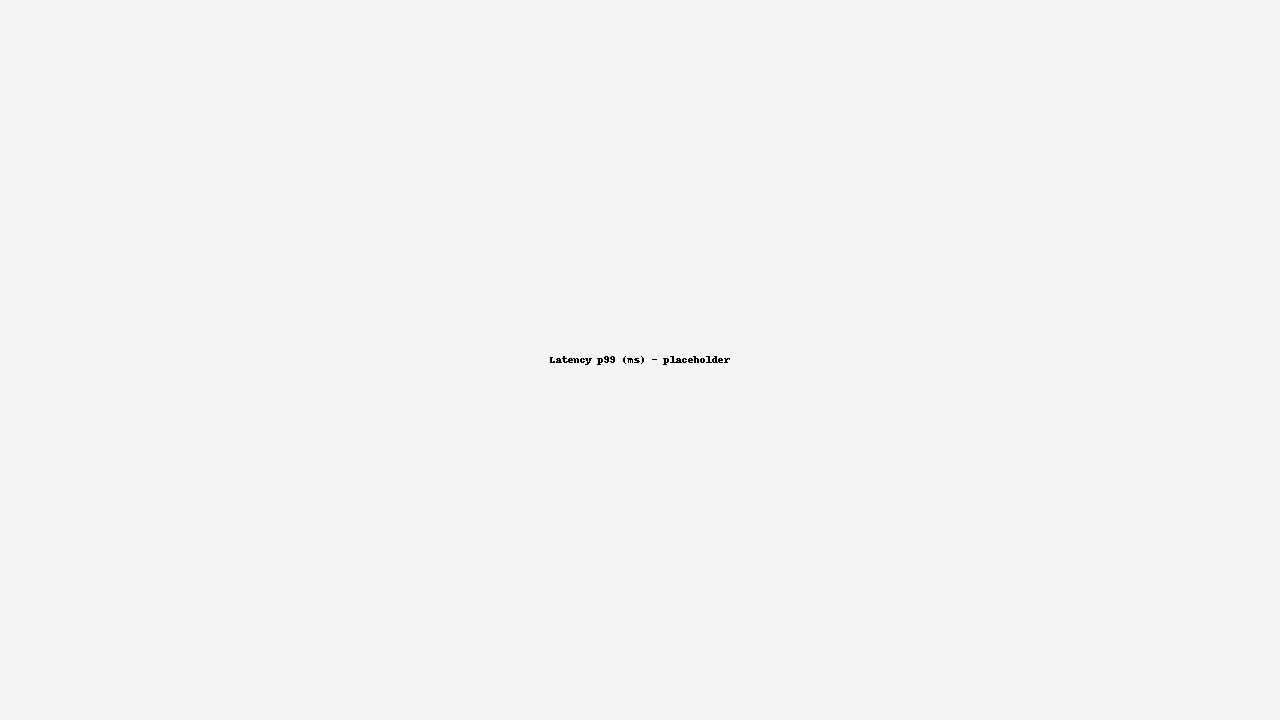
\includegraphics[width=\linewidth]{figures/latency_p99_ms.png}
\caption{Latency p99 (ms) across configurations.}\end{figure}

\begin{figure}[t]\centering

\includegraphics[width=\linewidth]{figures/throughput_eps.png}
\caption{Throughput (events/s).}\end{figure}

\section{Ablations and Sensitivity}



\textbf{Window size $W$.} Larger $W$ stabilizes thresholds but slows adaptation; smaller $W$ adapts faster but increases quantile variance. \\
\textbf{Target FPR $\alpha$.} Lower $\alpha$ reduces false alarms but may reduce TPR; $\alpha{=}0.01$ is a pragmatic default for operations. \\
\textbf{ADWIN $\delta$.} Smaller $\delta$ is more conservative (fewer false alarms) at the cost of slower shift detection. \\
\textbf{Transformer depth/width.} Shallow configurations often match or exceed Isolation Forest throughput while maintaining quality after calibration.

\section{Engineering Notes}

% --- AUTO-ADDED (Engineering Notes) ---
\paragraph{Calibration buffer.} We implement the sliding window as a fixed-size ring buffer and maintain the threshold with an approximate quantile structure (e.g., GK sketch) to avoid sorting at every step. On ADWIN signals we clear and warm-start the buffer to prevent stale thresholds.

\paragraph{Throughput and backpressure.} We default to one-at-a-time updates for predictable p95/p99 latency. Batch scoring improves CPU throughput but increases tail-latency variance; for strict SLOs we recommend batch size $=1$ with backpressure-aware ingestion.

\paragraph{Tokenization and hashing.} A hashed TF--IDF vectorizer avoids vocabulary blow-ups under template churn and enables constant-memory updates. For the transformer path we cap token length, prefer byte/character pieces for robustness, and freeze weights in streaming mode.

\paragraph{Reproducibility engineering.} CI is pinned by SHA, environments are lock-filed, and data integrity is tracked via size and SHA-256 in \texttt{data/HASHES.txt}. Scripts emit deterministic CSV rows and avoid wall-clock dependent randomness.
% --- END AUTO-ADDED ---


\section{Complexity and Memory}
\textbf{Baseline.} With a hashed TF--IDF vectorizer of dimension $d$ and IsolationForest of $T$ trees, scoring is $O(d)$ per line and model memory is $O(T \cdot \text{depth})$ (small for shallow trees). The sliding conformal buffer adds $O(W)$ memory; we maintain the threshold via a streaming quantile structure (binary heap or GK-sketch) to avoid full sorts.

\textbf{Transformer.} A micro-transformer with $L$ layers, hidden size $h$, and max token length $n$ yields $O(L \cdot n \cdot h^2)$ compute without KV caching. In practice we cap $n$ (truncate long lines) and prune width to stay within a few ms per line on commodity CPUs. Calibration and ADWIN overheads are negligible relative to the forward pass.

\textbf{Throughput.} End-to-end throughput is limited by featurization (tokenization + hashing), model scoring, and occasional calibrator updates. Batching can increase CPU efficiency but increases latency variance; we default to single-line updates for predictable p95/p99.





\textbf{Latency measurement.} Reported per-line timing includes tokenization, vectorization, scoring, conformal thresholding, and I/O. \\
\textbf{Masking.} Numeric fields and common identifiers are masked pre-vectorization to reduce spurious novelty from variable parts (e.g., PIDs, counters). \\
\textbf{Threading.} A lightweight pipeline can exploit batched featurization with micro-batching without changing conformal semantics.

\section{Threat Model and Operations}



\textbf{Adversarial inputs.} Attackers may inject rare templates to induce threshold drift. Conformal thresholds resist single outliers; ADWIN resets limit long-term damage. \\
\textbf{Privacy.} Logs may contain sensitive data even after masking. We recommend additional redaction and role-based access controls. \\
\textbf{Human-in-the-loop.} Anomalies should be triaged with feedback captured for future supervised refinement.

\section{Reproducibility Checklist}
\begin{itemize}[leftmargin=*]
  \item Deterministic seeds for featurization and model initialization.
  \item One canonical CSV row per run; 1:1 block in \texttt{docs/PROVENANCE.txt}.
  \item Artifact sizes and SHA-256 in \texttt{data/HASHES.txt} (uppercase).
  \item UTF-8 (no BOM), LF-only enforced by hooks; protected JSONs end without final LF.
  \item CI: pre-commit, mypy, CSV checks, tests on Windows and Ubuntu.
\end{itemize}

\section{Limitations and Ethics}

% --- AUTO-ADDED (Limitations and Ethics) ---
\paragraph{Limitations.} (i) After a drift reset the calibration buffer is short; quantile estimates are noisy for $<\!W$ steps. (ii) Synthetic labels are useful for smoke tests but not a substitute for real, delayed, and noisy labels. (iii) The transformer path, while compact, still costs more CPU than the sparse baseline; very high-throughput workloads may prefer the baseline.

\paragraph{Ethics and operations.} Log streams can contain sensitive information. This project does \emph{not} train models on private data; published datasets are synthetic or sanitized. We expose calibration targets and thresholds to avoid ``black-box'' alerting and provide reproducible procedures so others can audit results. In production, alerts should flow through a human-in-the-loop triage process with feedback for false positives.
% --- END AUTO-ADDED ---


\section{Responsible Release and Transparency}
We release code with (i) CI pinned by SHA, (ii) environment pins for reproducibility, and (iii) explicit data integrity via file size + SHA-256 in \texttt{data/HASHES.txt}. We avoid training or publishing models on sensitive data, document limitations (e.g., temporary FPR drift under abrupt distribution shifts), and provide a precise runbook so others can replicate results without hidden steps.


Synthetic datasets are small; production diversity and rare security payloads may be underrepresented. Conformal validity assumes short-term exchangeability; severe non-stationarity may require larger buffers or hybrid detectors. We mask dynamic fields but recommend layered redaction given privacy risks in logs.

\section{Conclusion and Future Work}
\balance


\subsection*{Summary}
A lightweight detector with sliding conformal calibration and ADWIN resets sustains a target FPR with predictable latency on commodity CPUs. In future work we will (i) add energy measurements when supported by hardware telemetry, (ii) explore character-level tokenization to reduce OOV effects, and (iii) provide a tiny distilled transformer variant with CPU-friendly kernels.


A compact, calibrated streaming pipeline with drift-aware resets provides competitive utility and strong reproducibility with an explicit audit trail. Future work: (i) template-aware tokenization, (ii) hybrid semi-supervision with weak labels, (iii) adaptive buffer sizing coupled to ADWIN confidence, and (iv) deployment studies on production traces.

\bibliographystyle{abbrv}
\bibliography{refs}
\end{document}
